%======================== 4. PROBLEM 3: VOLTAGES ===============================
\isec{\faBolt}{Problem 3: Motor Voltage Telemetry and Dynamics Logging}

\isub{\faCogs}{(i) Kinematics to wheel rates}
\begin{minipage}[c]{0.43\linewidth}
\centering
\begin{tikzpicture}[scale=0.82]
  \draw[kfupmdark,thick,fill=kfupmlight,rounded corners=4pt] (-1.6,-1.9) rectangle (1.6,1.9);
  \foreach \cx/\cy/\nm/\num in {-2.05/1.35/FL/2, 2.05/1.35/FR/1, -2.05/-1.35/RL/3, 2.05/-1.35/RR/4}{
    \fill[ink!80,rounded corners=2pt] (\cx-0.32,\cy-0.62) rectangle (\cx+0.32,\cy+0.62);
    \node[font=\small\bfseries,text=kfupmdark] at (\cx,\cy+0.9) {\nm\ ($\omega_{\num}$)};}
  % camera side at the top (+X)
  \fill[accred] (-0.35,1.9) rectangle (0.35,2.15);
  \node[font=\scriptsize,text=accred,above] at (0,2.15) {camera, gripper};
  \draw[-{Latex[length=2.6mm]},very thick,accblue] (0,0) -- (0,1.2) node[right,font=\small]{$+X$, $v>0$};
  \draw[-{Latex[length=2.6mm]},very thick,accblue] (0,0) -- (-1.2,0) node[above,font=\small]{$+Y$};
  \draw[-{Latex[length=2mm]},thick,accorange] (0.5,0) arc (0:250:0.5);
  \node[font=\small,text=accorange] at (0.82,-0.32) {$\omega_z$};
  \fill[ink] (0,0) circle (1.8pt);
  \draw[|<->|,muted] (0,-2.25) -- node[below,font=\small,text=ink]{$L_c=0.20$\,m} (2.05,-2.25);
  \node[font=\scriptsize,text=muted,align=center] at (0,-3.1) {wheel radius $r=0.05$\,m};
\end{tikzpicture}
\end{minipage}\hfill
\begin{minipage}[c]{0.55\linewidth}
\begin{keybox}{\faCogs\ \ Wheel rates (eq.~4)}
\vspace{-6pt}
\begin{equation}
\omega_1=\omega_4=\frac{v_x+L_c\,\omega_z}{r},\qquad
\omega_2=\omega_3=\frac{v_x-L_c\,\omega_z}{r}
\label{eq:wheels}
\end{equation}
\end{keybox}
\small
\begin{itemize}
  \item $1=$ FR, $2=$ FL, $3=$ RL, $4=$ RR. A counter-clockwise turn ($\omega_z>0$) speeds up the right side.
  \item It is the Mecanum inverse kinematics \cite{lynch} of Assessment~1 with $v_y=0$ and $l_x+l_y$ replaced by $L_c$. The
        A1 fit on logged data gave $R=51.0$\,mm and $l_x+l_y=204.7$\,mm, close to the $r$ and $L_c$ used here.
  \item Inputs are the \emph{commanded} $(v,\omega)$ in the mission frame, so $v>0$ (toward the tag) gives positive
        wheel rates.
\end{itemize}
\end{minipage}

\isub{\faBolt}{(ii) Motor armature voltage model}
\begin{keybox}{\faBolt\ \ Armature voltage (eq.~5), $K_v=0.38$\,V\,s/rad, $K_a=0.06$\,V\,s$^2$/rad}
\vspace{-6pt}
\begin{equation}
V_i(t)=\underbrace{K_v\,\omega_i(t)}_{\text{back-EMF}}+\underbrace{K_a\,\frac{\omega_i(t)-\omega_i(t-\Delta t)}{\Delta t}}_{\text{inertia}},
\qquad i\in\{1,2,3,4\},\qquad \Delta t=0.05\text{\,s}.
\label{eq:volt}
\end{equation}
\end{keybox}
\begin{itemize}
  \item \textbf{Where it runs:} inside the 20\,Hz control tick of \code{flatness_planner}, right after the command is
        published. $\Delta t$ is the control period; the logged tick interval was $50.0\pm0.3$\,ms (47 to 53\,ms) in
        the final run. The previous rates start at zero.
  \item \textbf{Which $\omega_i$:} the rates of eq.~(\ref{eq:wheels}) from the commanded $(v,\omega)$. The model gives
        the voltage the motors need to realize the command; it is not a measurement of the ESC terminals.
  \item \textbf{Steady values:} in a pure search turn ($\omega=0.30$\,rad/s) $|\omega_i|=1.2$\,rad/s and
        $|V_i|=0.38\times1.2=0.456$\,V. At the peak cruise speed (0.137\,m/s, $\omega_i=2.74$\,rad/s) the back-EMF term
        is about 1.04\,V.
  \item \textbf{Logging:} every tick goes to \code{motor_voltage_full.csv}; every 1\,s one row is printed to the
        terminal and written to \code{motor_voltage_log.csv} (the deliverable).
\end{itemize}

\begin{lstlisting}[style=py]
def wheel_rates(vx, wz, r=R_WHEEL, lc=L_C):
    """[w1, w2, w3, w4] in rad/s from forward speed vx (m/s) and yaw rate wz (rad/s, CCW +) (eq. 4)."""
    w_fr = (vx + lc * wz) / r
    w_fl = (vx - lc * wz) / r
    return np.array([w_fr, w_fl, w_fl, w_fr])


def motor_voltages(w, w_prev, dt, kv=K_V, ka=K_A):
    """V_i = Kv w_i + Ka (w_i - w_i_prev) / dt (eq. 5)."""
    w = np.asarray(w, dtype=float)
    return kv * w + ka * (w - np.asarray(w_prev, dtype=float)) / dt
\end{lstlisting}

\isub{\faTable}{(iii) Live table and CSV logging: Table 1}
Table~\ref{tab:table1} lists every row of \code{motor_voltage_log.csv} of the final run, as written by the planner
(target T3, start 1.50\,m, robot turned away from the tag). The terminal printed the same five columns live.
Unlike the template of the assignment, the log starts in SEARCHING, because T3 was placed outside the initial view
to demonstrate the sweep.

\begin{table}[H]
\centering\small
\setlength{\tabcolsep}{5.5pt}
\renewcommand{\arraystretch}{1.08}
\rowcolors{2}{kfupmlight}{white}
\begin{tabular}{@{}r rrrr rr r l@{}}
\rowcolor{kfupm}\hd{$t$ (s)} & \hd{$V_1$ (V)} & \hd{$V_2$ (V)} & \hd{$V_3$ (V)} & \hd{$V_4$ (V)} & \hd{$v$ (m/s)} & \hd{$\omega$ (rad/s)} & \hd{$d$ (m)} & \hd{State}\\
% Generated by analysis/plot_voltage.py from data/runs/20261026_015001/motor_voltage_log.csv.
% Values copied verbatim (strings), do not edit by hand.
0 & 1.896 & $-1.896$ & $-1.896$ & 1.896 & 0.0000 & 0.3000 & n/a & \stbadge{SEARCHING}\\
1 & 0.456 & $-0.456$ & $-0.456$ & 0.456 & 0.0000 & 0.3000 & n/a & \stbadge{SEARCHING}\\
2 & 0.456 & $-0.456$ & $-0.456$ & 0.456 & 0.0000 & 0.3000 & n/a & \stbadge{SEARCHING}\\
3 & 0.456 & $-0.456$ & $-0.456$ & 0.456 & 0.0000 & 0.3000 & n/a & \stbadge{SEARCHING}\\
4 & 0.456 & $-0.456$ & $-0.456$ & 0.456 & 0.0000 & 0.3000 & n/a & \stbadge{SEARCHING}\\
5 & 0.456 & $-0.456$ & $-0.456$ & 0.456 & 0.0000 & 0.3000 & n/a & \stbadge{SEARCHING}\\
6 & 0.456 & $-0.456$ & $-0.456$ & 0.456 & 0.0000 & 0.3000 & 1.273 & \stbadge{ALIGNING}\\
7 & 0.456 & $-0.456$ & $-0.456$ & 0.456 & 0.0000 & 0.3000 & 1.300 & \stbadge{SEARCHING}\\
8 & 0.456 & $-0.456$ & $-0.456$ & 0.456 & 0.0000 & 0.3000 & 1.300 & \stbadge{SEARCHING}\\
9 & 0.583 & 0.583 & 0.583 & 0.583 & 0.0725 & 0.0000 & 1.440 & \stbadge{CHASING}\\
10 & 0.750 & 0.750 & 0.750 & 0.750 & 0.0953 & 0.0000 & 1.440 & \stbadge{CHASING}\\
11 & $-0.437$ & 0.437 & 0.437 & $-0.437$ & 0.0000 & $-0.2878$ & 1.267 & \stbadge{ALIGNING}\\
12 & 0.552 & 0.652 & 0.652 & 0.552 & 0.0744 & $-0.0532$ & 1.288 & \stbadge{CHASING}\\
13 & 0.847 & 0.729 & 0.729 & 0.847 & 0.1000 & 0.0222 & 1.193 & \stbadge{CHASING}\\
14 & 0.952 & 0.916 & 0.916 & 0.952 & 0.1205 & 0.0118 & 1.101 & \stbadge{CHASING}\\
15 & 1.029 & 1.005 & 1.005 & 1.029 & 0.1324 & 0.0067 & 0.963 & \stbadge{CHASING}\\
16 & 1.063 & 1.024 & 1.024 & 1.063 & 0.1371 & 0.0062 & 0.836 & \stbadge{CHASING}\\
17 & 0.997 & 1.031 & 1.031 & 0.997 & 0.1344 & 0.0036 & 0.690 & \stbadge{CHASING}\\
18 & 0.931 & 0.926 & 0.926 & 0.931 & 0.1243 & 0.0043 & 0.572 & \stbadge{CHASING}\\
19 & 0.807 & 0.784 & 0.784 & 0.807 & 0.1079 & 0.0074 & 0.456 & \stbadge{CHASING}\\
20 & 0.544 & 0.636 & 0.636 & 0.544 & 0.0821 & 0.0000 & 0.391 & \stbadge{CHASING}\\
21 & 0.337 & 0.337 & 0.337 & 0.337 & 0.0500 & 0.0000 & 0.391 & \stbadge{CHASING}\\
22 & 0.028 & 0.028 & 0.028 & 0.028 & 0.0105 & 0.0000 & 0.391 & \stbadge{CHASING}\\
23 & 0.000 & 0.000 & 0.000 & 0.000 & 0.0000 & 0.0000 & 0.391 & \stbadge{ARRIVED}\\
24 & 0.000 & 0.000 & 0.000 & 0.000 & 0.0000 & 0.0000 & 0.391 & \stbadge{ARRIVED}\\
25 & 0.000 & 0.000 & 0.000 & 0.000 & 0.0000 & 0.0000 & 0.391 & \stbadge{ARRIVED}\\

\end{tabular}
\caption{Chassis motor armature voltage log, target Tag 3, final run \code{20261026_015001} (verbatim rows of
\code{motor_voltage_log.csv}). $v$, $\omega$ are the commanded values of that tick. $d$ is the last camera range
received (it holds its value while T3 is not seen, and n/a before the first detection). $T_{stop}=22.30$\,s; from
$t=23$\,s all four voltages are 0.000\,V.}
\label{tab:table1}
\end{table}

\begin{figure}[H]
\centering
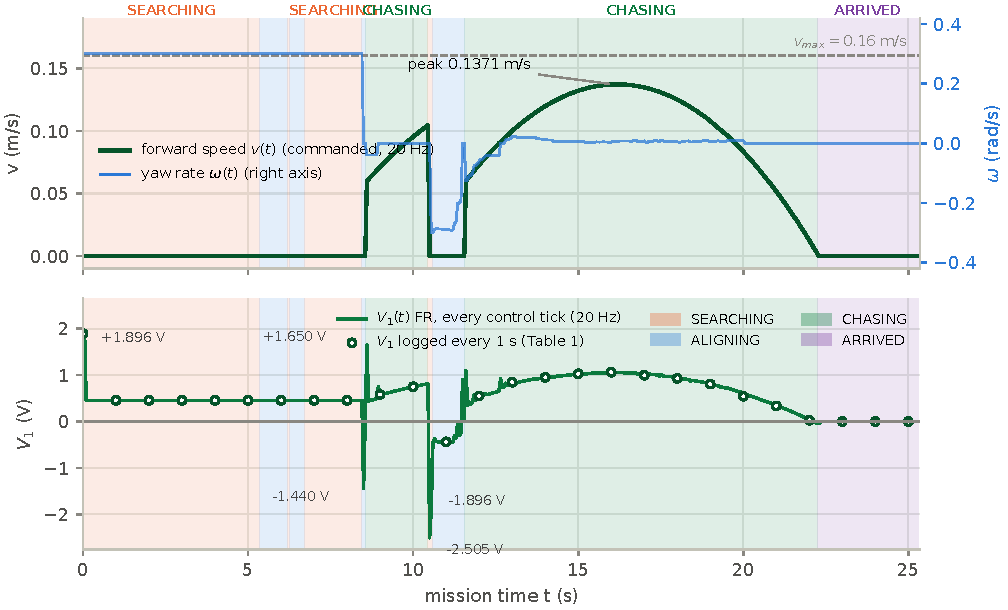
\includegraphics[width=\linewidth]{figures/p3_v_V1.pdf}
\caption{Forward speed $v(t)$ and motor voltage $V_1(t)$ (front right) over the final run, with the state machine
colored in the background. Top: commanded $v$ and $\omega$ at 20\,Hz. Bottom: $V_1$ at every control tick (line) and
the 1\,s rows of Table~\ref{tab:table1} (circles).}
\label{fig:vV1}
\end{figure}

\begin{figure}[H]
\centering
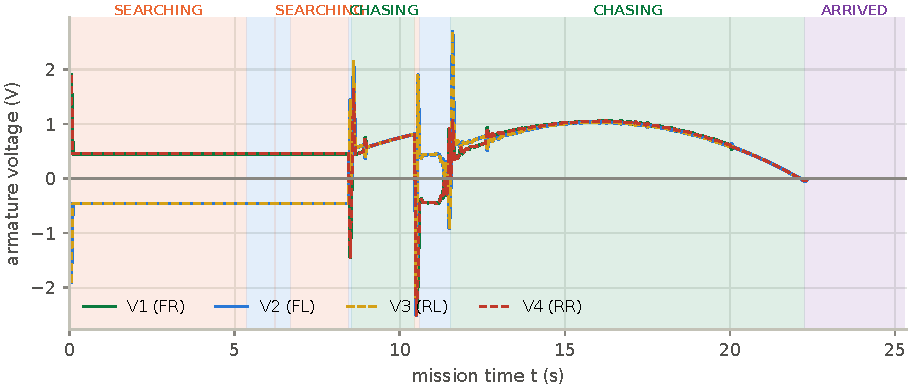
\includegraphics[width=\linewidth]{figures/p3_voltages_all.pdf}
\caption{All four armature voltages at 20\,Hz. Left and right pairs are equal ($V_1=V_4$, $V_2=V_3$) because eq.~(4)
has no lateral term; they differ only when $\omega\neq0$.}
\label{fig:vall}
\end{figure}

\begin{purplebox}{\faSearch\ \ Reading the voltage log}
\small
\begin{itemize}
  \item \textbf{Zero after the halt (confirmed).} The 1\,s rows at $t=23$, 24 and 25\,s are 0.000\,V on all motors. At
        20\,Hz the first ARRIVED tick (22.30\,s) carries $-0.041$\,V, the inertia term of the last speed decrement;
        the remaining 60 ticks are exactly 0.000\,V.
  \item \textbf{Search turn} (Figure~\ref{fig:vall}): $V_1=V_4=+0.456$\,V, $V_2=V_3=-0.456$\,V: the right side drives forward, the left side
        backward, the robot turns counter-clockwise.
  \item \textbf{Spikes are steps of the command.} Eq.~(\ref{eq:volt}) differentiates the command over one 50\,ms tick,
        so every step adds $K_a\Delta\omega_i/\Delta t$ for one tick:
        \begin{itemize}
          \item $t=0$: $0\rightarrow1.2$\,rad/s, $0.456+0.06\times1.2/0.05=\mathbf{1.896}$\,V (the first row of
                Table~\ref{tab:table1});
          \item 8.50\,s, centered: the turn stops, $-1.440$\,V on $V_1$;
          \item 8.60 and 11.60\,s, CHASING starts at $\dot x(0)=0.06$\,m/s (a step required by the boundary
                condition) plus the bearing correction: up to $+2.694$\,V on $V_2$;
          \item 10.50\,s, detection gap: the chase drops from 0.104\,m/s to rest, $-2.505$\,V on all motors.
        \end{itemize}
  \item \textbf{Smooth cruise.} Inside the plan the planned acceleration ($|\ddot x|\le0.045$\,m/s$^2$) adds at most $0.06\times0.0449/0.05=0.054$\,V; small
        changes of the bearing correction add up to 0.23\,V on single wheels. $V_1$ follows the speed profile and
        peaks at 1.063\,V in the $t=16$\,s row.
  \item \textbf{Negative voltage while braking.} In the last three CHASING ticks (22.15 to 22.25\,s) the deceleration
        term outweighs the back-EMF of the nearly stopped wheels: $-0.006$, $-0.023$, $-0.040$\,V. The motors oppose
        the motion: braking, which a real drive can do regeneratively.
  \item \textbf{Left and right voltages differ only while turning} or in the tick where a turn stops
        (rows 11 to 20: re-alignment and bearing correction, $|\omega|\le0.29$\,rad/s).
\end{itemize}
\end{purplebox}
